\section{Profil Management}
\setauthor{David Hauser}
\section{Webshop}
\setauthor{Benjamin Golic}
\section{Automatic Number Plate Recognition (ANPR)[SK]}
\setauthor{Simon Koll}
\label{lsg:def:anpr}
Die Kennzeichenerkennung stellt das Alleinstellungsmerkmal des Projektes dar. Der OpenCV-Python-Code für die Nummernschilderkennung umfasst drei Hauptschritte. Der erste Schritt ist die Erkennung von Nummernschildern. Die Konturfunktion wird verwendet, um die rechteckigen Objekte im Bild zu erkennen und das Nummernschild zu finden. Der zweite Schritt ist die Zeichensegmentierung. Sobald die Kontur das Nummernschild erkannt wurde, muss es ausgeschnitten und als neues Bild gespeichert werden. Der letzte Schritt ist die Zeichenerkennung. Die optische Zeichenerkennung wird auf dem ausgeschnittenen Bild durchgeführt, um das Kennzeichen zu erkennen.

\subsection{Überprüfung der Kennzeichen}
Die erkannten Buchstaben werden genutzt, um eine Funktion aufzurufen, welche diese mit den zugelassenen Kennzeichen vergleicht. Dazu werden die zugelassenen Kennzeichen vom Server abgefragt, welcher diese aus der Datenbank lädt. Die Abfrage erfolgt über eine REST-Abfrage.
REST ist weder ein Protokoll, noch ein Standard. REST steht für REpresentational State Transfer, API für Application Programming Interface, welche gemeinsam eine Programmierschnittstelle bilden, mit der Anwendungen mit einem Server kommunizieren können. Dies wird meist mit dem HTTP-Protokoll genutzt, um Services über URLs zu erreichen. Dazu stehen die HTTP-Methoden GET, POST, PUT und DELETE zur Verfügung.
\begin{itemize}
    \item \textit{GET: } GET ist eine Methode, welche einen Inhalt eines Servers abruft.
    \item \textit{POST: } POST ist eine Methode, um vom Client Daten an den Server zu senden, welcher diese weiter verarbeiten und in die Datenbank speichern kann.
    \item \textit{PUT: } PUT bietet die Möglichkeit, bereits bestehende Daten zu ändern.
    \item \textit{DELETE: } DELETE bietet die Möglichkeit, bestehende Daten zu löschen.
\end{itemize}\cite{WhatIsREST}
Neben der Kennzeichenerkennung bietet das Projekt noch 2 weitere Zutrittsmöglichkeit, nämlich das Nummernfeld sowie die NFC-Funktionalität. Damit alle Zutrittsmöglichkeiten parallel funktionieren, wird mit der Bibliothek \textit{threading} parallel gearbeitet. Hiermit können mehrere Funktionen parallel gestartet werden. Dies kann beispielsweise wie folgt erfolgen: 
\begin{lstlisting}[language=Python, caption=Funktionsweise von Multiprocessing, label=lst:lsg:multiprocessing]
import time
from threading import Thread
    def funktion_1():
        while True:
            print("Funktion 1")
            time.sleep(1)
    
    
    def funktion_2():
        while True:
            print("Funktion 2")
            time.sleep(1)
    
    
    thread_1 = Thread(target=funktion_1)
    thread_2 = Thread(target=funktion_2)
    
    thread_1.start()
    thread_2.start()
\end{lstlisting}
\verb|thread_1| und \verb|thread_2| sind Threads, welche parallel ausgeführt werden. Sie bekommen als Parameter eine Funktion, welche ausgeführt werden soll, in diesem Fall \verb|funktion_1| und \verb|funktion_2|. Mit \verb|start()| werden die Threads gestartet.
    \cite{threading}
\section{Backend}
\setauthor{Simon Koll}
Der Server bildet das Rückgrat des Projektes. Hier werden die Daten aus der Datenbank abgefragt. Diese werden von einem Client über einen REST-Aufruf abgefragt. Der Server kann zudem die neu zugelassenen Kennzeichen in die Datenbank speichern.
\subsection{Oracle VM}
Der Server läuft auf einer Instanz einer Oracle Virtual Machine, ebenso die MongoDB-Datenbank. Die Oracle VM bietet die Möglichkeit, eine leistungsstarke Basis für den Server sowie für die Datenbank bereitzustellen. Die technischen Daten der Instanz sind:
\begin{table}[ht]
    \caption{Technische Daten der Oracle VM Instanz}
    \label{tab:vm}
    \begin{tabular}{|l|llll}
    \cline{1-2}
    \textbf{Komponente} & \multicolumn{1}{l|}{\textbf{Wert}} &  &  &  \\ \cline{1-2}
    \textbf{CPU}        & 2 OCPU                             &  &  &  \\ \cline{1-1}
    \textbf{RAM}        & 16 GB                              &  &  &  \\ \cline{1-1}
    \textbf{Netzwerk}   & 1.4 GBit Bandbreite                &  &  &  \\ \cline{1-1}
    \end{tabular}
    \end{table}

    Im Vergleich zu anderen Cloudanbietern wie AWS, Microsoft oder Google, verwendet die Oracle Cloud Infrastructure, kurz OCI, anstelle von virtuellen CPUs sogenannte OCPUs. Jede vCPU ist als ein Hyperthread eines Intel Xeon-Kerns definiert. Ein Standard-Intel-Prozessorkern mit aktiviertem Hyperthreading hat 2 Threads.
\begin{figure}[H]
    \centering
    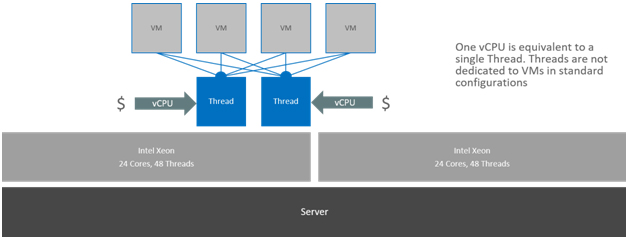
\includegraphics[width=0.8\textwidth]{pics/vCPU.jpg}
    \caption{Visualisierung von vCPUs}
    \cite{vcpuPic}
    \label{fig:vm:vCPU}
\end{figure}

    Eine OCPU ist definiert als die CPU-Kapazität, die einem physischen Kern eines Intel Xeon-Prozessors mit aktiviertem Hyperthreading oder einem physischen Kern eines Oracle SPARC-Prozessors entspricht.
    \begin{figure}[H]
        \centering
        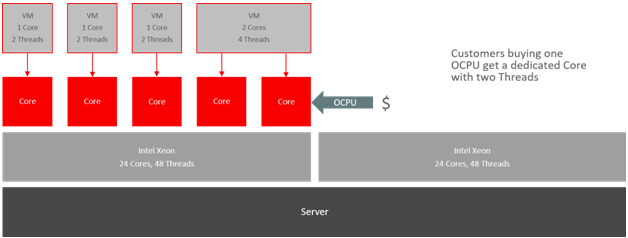
\includegraphics[width=0.8\textwidth]{pics/OCPU.jpg}
        \caption{Visualisierung von OCPUs}
        \cite{ocpuPic}
        \label{fig:vm:OCPU}
    \end{figure}
\cite{vcpuVsocpu}
\section{MongoDB}
Die Datenbank läuft auf der selben Oracle VM Instanz wie das Backend. Somit gibt es zwischen Server und Datenbank keine zusätzliche Latenz. Da MongoDB eine nicht relationale Datenbank ist, werden die Daten in sogenannten Collections anstelle von Tabellen abgespeichert. Je nach abzuspeichernder Zugangsmöglichkeit, verändert sich das Format der Daten.
Für ein Kennzeichen müssen die Daten wie folgt strukturiert sein:

\subsubsection{Kennzeichen}
\begin{lstlisting}[language=JSON, caption=Aufbau eines Kennzeichen in der Datenbank, label=lst:lsg:licenseplate]
    {
        "_id": "623f449cb8c1b2f4f64c4351",
        "licenseplate_id": 1,
        "licenseplate": "RO 108DV",
        "time_created": 1647252201,
        "active": true
    }
\end{lstlisting}
Das Attribut \verb|_id| wird automatisch generiert und ist ein eindeutiger Schlüssel, welcher die eindeutige Identifizierung eines Datensatzes darstellt. Mithilfe des \verb|licenseplate_id| wird eine eindeutige Kennzeichen Identifikationsnummer gespeichert. \verb|licenseplate| ist das Kennzeichen, welches vom Client übergeben wurde. \verb|time_created| ist die Zeit, zu der das Kennzeichen erstellt wurde. \verb|active| gibt an, ob das Kennzeichen der aktiv ist.

\subsubsection{Nummernfeld}
Bei einer Nummernfeld-Kombination sieht der Datensatz wie folgt aus:
\begin{lstlisting}[language=JSON, caption=Aufbau einer Nummernfeld-Kombination in der Datenbank, label=lst:lsg:numpad]
    {
        "_id": "622f181d35a3c2ce232acad9",
        "numpad_id": 1,
        "numpad_code": "123456",
        "time_created": 1647252201,
        "active": true
    }
\end{lstlisting}

\subsubsection{NFC}
Jede NFC-Karte hat eine eindeutige, 10-stellige Kartenidentifikationsnummer. Diese kann mittels eines RFID-Lesers ausgelesen werden. In der Datenbank werden die NFC-Informationen wie folgt gespeichert:
\begin{lstlisting}[language=JSON, caption=Aufbau einer NFC-Karte in der Datenbank, label=lst:lsg:nfc]
    {
        "_id": "622f781cfbd4e8de471a4035",
        "rfid_id": 3,
        "rfid_code": "01928384756",
        "time_created": "123456789",
        "active": true
    }
    \end{lstlisting}